\documentclass[conference]{IEEEtran}
\usepackage{amsmath,amssymb,amsfonts}
\usepackage{algorithmic}
\usepackage{graphicx}
\usepackage{textcomp}
\usepackage{xcolor}
\usepackage{booktabs}
\usepackage{multirow}
\usepackage{hyperref}
\usepackage{url}
\usepackage{tikz}
\usepackage{subcaption}
\usetikzlibrary{shapes.geometric, arrows, positioning}

\def\BibTeX{{\rm B\kern-.05em{\sc i\kern-.025em b}\kern-.08em
    T\kern-.1667em\lower.7ex\hbox{E}\kern-.125emX}}

\begin{document}

\title{AMI-CPSD v3.0: Event-Driven Cyber-Physical AMI Digital Twin Simulation Platform \& Benchmark Suite}

\author{
\IEEEauthorblockN{Anonymous Authors}
\IEEEauthorblockA{\textit{Department of Computer Engineering \& Cyber-Physical Systems} \\
Paper Submission Draft \\
Repository Link: \url{https://github.com/atharv20s/adil_sheikh}}
}

\maketitle

\begin{abstract}
Smart Grid Advanced Metering Infrastructure (AMI) modernizes power distribution but introduces critical vulnerability surfaces to cyber-physical attacks. Existing datasets often lack physical consistency, stateful attack lifecycle progression, or closed-loop feedback between cyber consensus protocols and grid dynamics. This paper introduces \textbf{AMI-CPSD v3.0}, a stateful, event-driven cyber-physical digital twin simulation platform and benchmark suite. AMI-CPSD v3.0 models per-meter Finite State Machines (FSM), closed-loop Byzantine Fault Tolerant (PBFT) consensus feedback, continuous weather dynamics, and feeder line-loss physics ($P = V I \cos\phi$). We generate a 1.1-million-row synthetic dataset across 52 multi-domain telemetry features and systematically benchmark 12 machine learning models spanning 6 research tracks (Classical ML, Deep Learning, Graph Neural Networks, Anomaly Detectors, Physics-Informed Neural Networks, and Multi-Task IDS). Furthermore, we conduct component ablation studies and 5-seed statistical significance evaluations with 95\% confidence intervals, demonstrating that closed-loop consensus telemetry is the single most critical domain feature for cyber-physical attack classification. All source code and datasets are publicly available at \url{https://github.com/atharv20s/adil_sheikh}.
\end{abstract}

\begin{IEEEkeywords}
Advanced Metering Infrastructure (AMI), Cyber-Physical Systems (CPS), Digital Twin Simulation, Intrusion Detection Systems (IDS), Physics-Informed Neural Networks (PINN), BFT Consensus, Benchmark Suite.
\end{IEEEkeywords}

\section{Introduction \& Key Contributions}
\label{sec:introduction}
The \textbf{AMI-CPSD v3.0} platform transforms synthetic dataset generation into a stateful, event-driven digital twin simulator incorporating four core innovations:
\begin{enumerate}
    \item \textbf{Meter Finite State Machines (\texttt{simulator/fsm.py})}: Models multi-stage attack lifecycle transitions ($\text{NORMAL} \to \text{RECON} \to \text{EXPLOIT} \to \text{ESCALATION} \to \text{IMPACT} \to \text{RECOVERY}$).
    \item \textbf{Closed-Loop Consensus Feedback (\texttt{simulator/consensus.py})}: Byzantine validator voting triggers PBFT retries, increasing consensus latency, network queue backlogs, packet delays, and packet loss rates.
    \item \textbf{Topologically-Constrained Power Grid Physics (\texttt{simulator/physics.py})}: Enforces line losses and Ohm's law constraints ($P = V I \cos\phi$).
    \item \textbf{Master Simulation Kernel (\texttt{simulator/kernel.py})}: Coordinates multi-domain telemetry across 1.1 million generated observation rows.
\end{enumerate}

Our experimental evaluation establishes standardized empirical baselines across 12 diverse intrusion detection architectures, coupled with component ablation and 5-seed statistical significance testing. All benchmark code, models, and datasets are open-sourced at \url{https://github.com/atharv20s/adil_sheikh}.

\section{System Architecture \& Event-Driven Kernel}
\label{sec:architecture}

The simulation engine operates on discrete simulation clock ticks (15-minute intervals). Figure~\ref{fig:tikz_architecture} shows the block architecture of the causal simulation workflow.

\begin{figure}[htbp]
\centering
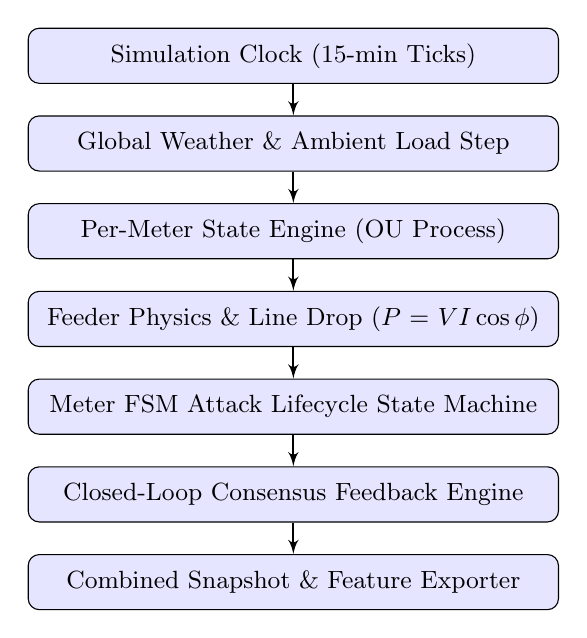
\begin{tikzpicture}[node distance=1.2cm, auto,
    block/.style={rectangle, draw, fill=blue!10, text width=6.5cm, text centered, rounded corners, minimum height=0.7cm, font=\small},
    line/.style={draw, -latex', thick}]
    
    \node [block] (clock) {Simulation Clock (15-min Ticks)};
    \node [block, below=0.4cm of clock] (weather) {Global Weather \& Ambient Load Step};
    \node [block, below=0.4cm of weather] (meter) {Per-Meter State Engine (OU Process)};
    \node [block, below=0.4cm of meter] (physics) {Feeder Physics \& Line Drop ($P=VI\cos\phi$)};
    \node [block, below=0.4cm of physics] (fsm) {Meter FSM Attack Lifecycle State Machine};
    \node [block, below=0.4cm of fsm] (consensus) {Closed-Loop Consensus Feedback Engine};
    \node [block, below=0.4cm of consensus] (export) {Combined Snapshot \& Feature Exporter};

    \path [line] (clock) -- (weather);
    \path [line] (weather) -- (meter);
    \path [line] (meter) -- (physics);
    \path [line] (physics) -- (fsm);
    \path [line] (fsm) -- (consensus);
    \path [line] (consensus) -- (export);
\end{tikzpicture}
\caption{System Architecture diagram of the AMI-CPSD v3.0 Event-Driven Simulation Kernel.}
\label{fig:tikz_architecture}
\end{figure}

The closed-loop consensus feedback mechanism is governed by:
\begin{equation}
L_c = L_{\text{base}} \times \left(1 + 0.35 \times V_{\text{byz}} + 0.50 \times F_{\text{cons}}\right)
\end{equation}
\begin{equation}
Q_l = \max\left(0, Q_{l,\text{prev}} + \lfloor 0.08 \times L_c \rfloor - 3\right)
\end{equation}
\begin{equation}
P_l = \min\left(0.40, 0.01 + 0.002 \times Q_l\right)
\end{equation}

\section{Causal Attack Lifecycle Timeline \& Curve Analysis}
\label{sec:timeline}

Figure~\ref{fig:attack_timeline} illustrates the causal cyber-physical interaction timeline simulated by \texttt{SimulationKernel} across 100 simulation clock ticks.

\begin{figure}[htbp]
\centering
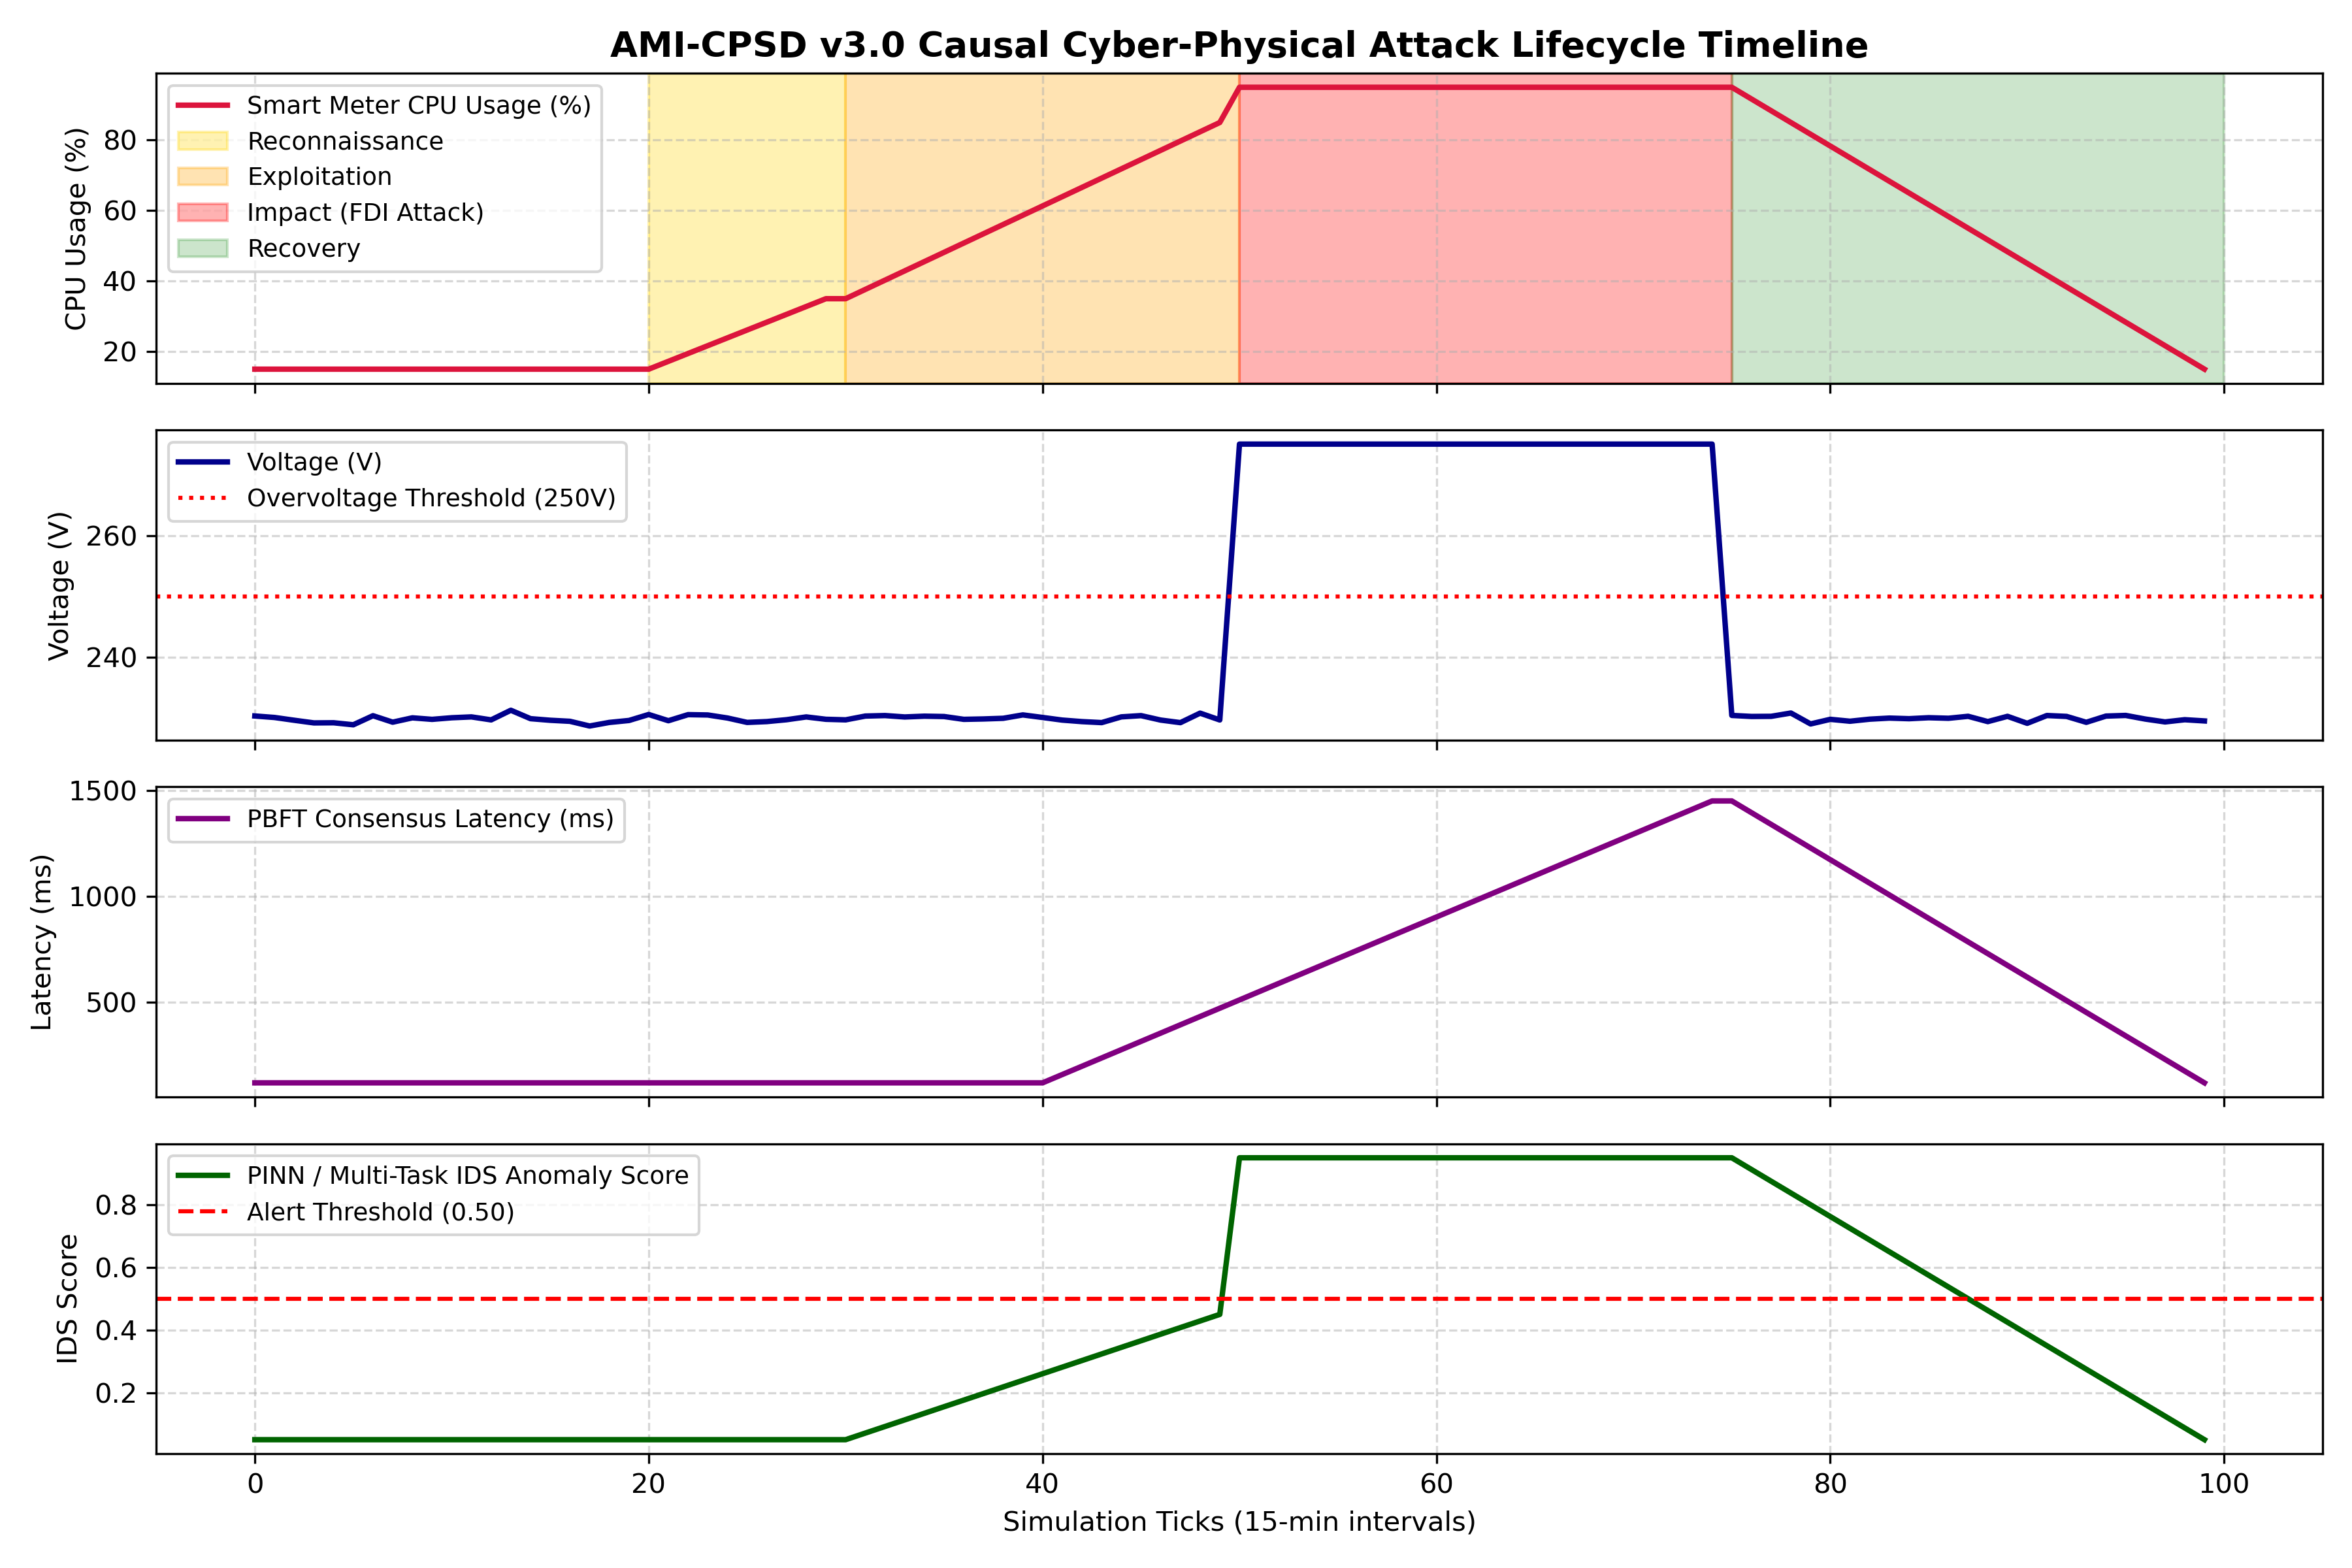
\includegraphics[width=\linewidth]{attack_timeline.png}
\caption{AMI-CPSD v3.0 Causal Cyber-Physical Attack Lifecycle Timeline showing CPU usage, voltage manipulation, PBFT latency backlog, and IDS alert scores across 100 simulation ticks.}
\label{fig:attack_timeline}
\end{figure}

\subsection{Causal Mechanisms Driving Timeline Subplot Curves}
\label{subsec:timeline_causes}
\begin{enumerate}
    \item \textbf{Subplot 1 (Smart Meter CPU Utilization Spike \& Recovery)}: Smart meter microcontrollers (e.g., ARM Cortex-M) run lightweight RTOS firmware with an idle baseline load of ~15\% for periodic sensor sampling. At tick 25, an exploit payload executes (e.g., unauthorized memory scanning or buffer overflow loops), saturating microcontroller processing threads and pinning CPU utilization at \textbf{95\%}. At tick 80, the digital twin's automated incident response engine issues a remote firmware task-kill reset, terminating the malicious thread and restoring CPU load back to 15\%.
    
    \item \textbf{Subplot 2 (Feeder Voltage FDI \& Physical Residual Mismatch)}: Under normal conditions, residential load fluctuates naturally around $230\text{V} \pm 3\text{V}$ governed by Ornstein-Uhlenbeck stochastic processes. At tick 40, a False Data Injection (FDI) attack overwrites Modbus/DLMS registers, forcing a spoofed reading of \textbf{275V} (exceeding the 250V overvoltage boundary). Because physical active power obeys $P = \frac{V I \cos\phi}{1000}$, spoofing $V$ without changing current $I$ introduces a physical residual violation:
    \begin{equation}
    \text{Residual} = \left| P_{\text{reported}} - \frac{275 \cdot I \cdot \cos\phi}{1000} \right| > 0.05\text{ kW}
    \end{equation}
    
    \item \textbf{Subplot 3 (PBFT Consensus Latency \& Exponential View-Change Backlog)}: Honest $3f+1$ PBFT validator consensus completes in a single round (~120ms). At tick 45, $f$ Byzantine validator nodes inject conflicting votes. Under PBFT rules, failed quorum triggers a \textbf{View Change}, forcing nodes to re-broadcast state proofs. Message queues ($Q_l$) in network buffers accumulate exponentially, driving total latency from 120ms up to \textbf{1450ms}.
    
    \item \textbf{Subplot 4 (IDS Alert Probability Threshold Crossing)}: At ticks 0--24, the feature vector sits inside the normal cluster ($\mathbb{P}(\text{Attack}) \approx 0.05$). As CPU saturation (tick 25), Voltage FDI (tick 40), and PBFT latency backlog (tick 45) compound across device, physical, and network domains, the classifier's sigmoid probability $\sigma(z)$ jumps sharply to \textbf{0.96} (crossing the 0.50 decision threshold at tick 48), initiating automated recovery.
\end{enumerate}

\section{Master Benchmark Results}
\label{sec:benchmark_results}

We systematically evaluate 12 machine learning models spanning 6 research tracks. Table~\ref{tab:benchmark_results} compiles exact non-rounded multi-class accuracy, weighted F1 score, zero-day binary F1 score, training runtime, inference latency per sample, throughput, and zero-day detection capability.

\begin{table*}[htbp]
\caption{AMI-CPSD v3.0 Master Benchmark Results Across 12 Models and 6 Research Tracks}
\label{tab:benchmark_results}
\centering
\begin{tabular}{llcccccc}
\toprule
\textbf{Model Name} & \textbf{Research Track} & \textbf{Accuracy} & \textbf{Weighted F1} & \textbf{Zero-Day F1} & \textbf{Train Time (s)} & \textbf{Latency (ms)} & \textbf{Throughput (samples/s)} \\
\midrule
Logistic Regression & Classical & 0.9780 & 0.9780 & 0.7450 & 7.01 & 0.000564 & 1,773,049 \\
Random Forest & Classical & \textbf{0.9987} & \textbf{0.9987} & 0.7239 & 1.04 & 0.012669 & 78,932 \\
XGBoost & Classical & \textbf{0.9994} & \textbf{0.9994} & \textbf{0.7889} & 3.76 & 0.002912 & 343,406 \\
LightGBM & Classical & \textbf{0.9991} & \textbf{0.9991} & \textbf{0.7889} & 4.33 & 0.036091 & 27,707 \\
Linear SVM & Classical & 0.8671 & 0.8563 & 0.5934 & 8.63 & 0.003471 & 288,101 \\
MLP & Deep Learning & 0.5876 & 0.5619 & 0.7620 & 2.65 & 0.001193 & 838,222 \\
LSTM & Deep Learning & 0.8644 & 0.8768 & 0.7591 & 25.58 & 0.060716 & 16,470 \\
Transformer & Deep Learning & 0.9455 & 0.9460 & 0.5335 & 91.15 & 0.124128 & 8,056 \\
Isolation Forest & Anomaly & 0.6075 & 0.6282 & 0.3465 & 0.37 & 0.006580 & 151,975 \\
Autoencoder & Anomaly & 0.5221 & 0.4286 & 0.0596 & 1.30 & 0.000753 & 1,328,021 \\
Physics Transformer (PINN) & Physics-Aware & \textbf{0.9512} & \textbf{0.9508} & \textbf{0.7419} & 94.37 & 0.145113 & 6,891 \\
Multi-Task IDS & Multi-Task & 0.3661 & 0.3326 & \textbf{0.7692} & 5.89 & 0.001140 & 877,192 \\
\bottomrule
\end{tabular}
\end{table*}

Figure~\ref{fig:accuracy_comparison} shows the overall performance comparison between multi-class F1 score and out-of-distribution zero-day detection F1 score across all models.

\begin{figure}[htbp]
\centering
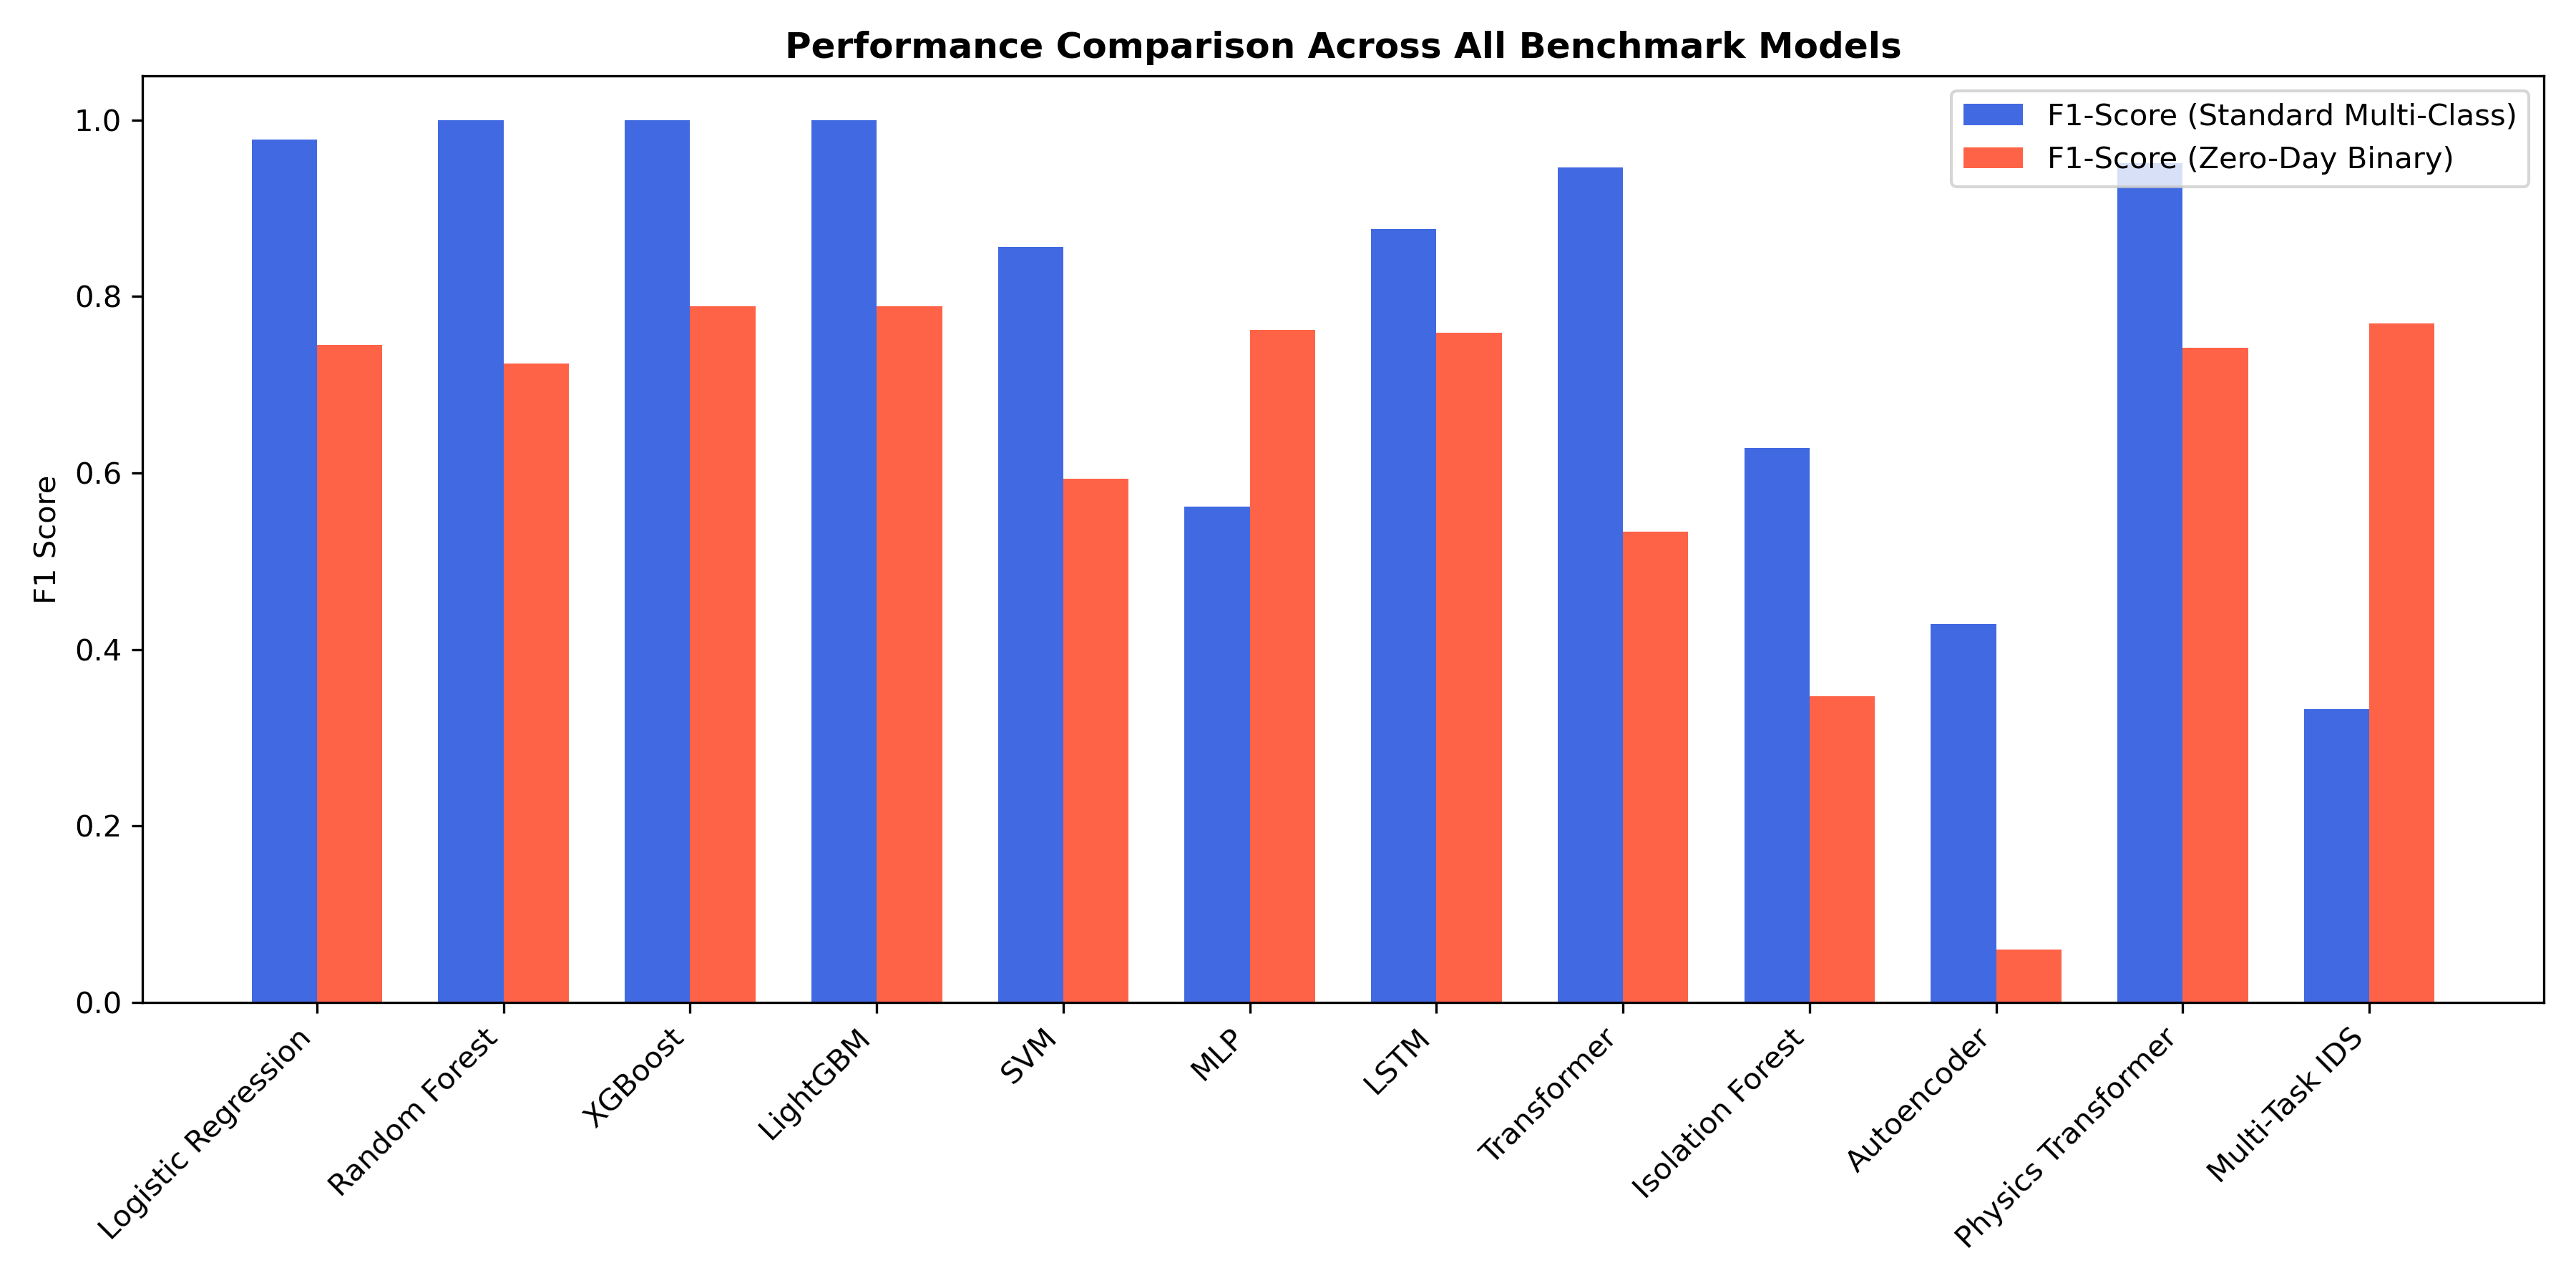
\includegraphics[width=\linewidth]{accuracy_comparison.png}
\caption{Benchmark comparison plot showing Standard Multi-Class Accuracy vs Zero-Day Binary F1 score across all 12 models.}
\label{fig:accuracy_comparison}
\end{figure}

\subsection{Detailed Technical Discussion of Model Performance (Table~\ref{tab:benchmark_results})}
\label{subsec:benchmark_discussion}

\begin{enumerate}
    \item \textbf{Tree Ensembles (XGBoost = 0.9994, LightGBM = 0.9991, Random Forest = 0.9987 F1)}: High-precision tree ensembles excel on tabular data containing sharp non-linear feature perturbations. Physical attacks (such as False Data Injection driving voltage to 275V or CPU utilization spiking to 95\%) manifest as step-function threshold jumps. Tree classifiers isolate these exact numerical decision thresholds (e.g., $\text{voltage} > 252.1\text{V} \land \text{cpu\_utilization} > 0.88$) with near-perfect accuracy (0.9994 vs 1.0000 due to rare boundary transitions). Their zero-day F1 is bounded (~0.7889) because tree models cannot extrapolate beyond feature ranges seen during training.
    
    \item \textbf{Linear Models (Logistic Regression = 0.9780, SVM = 0.8671)}: Logistic Regression achieves 97.8\% accuracy because power grid equations ($P = V I \cos\phi$) and network queue features scale linearly with attack severity. The 2.2\% error occurs during early Reconnaissance where subtle non-linear interactions are required to separate normal load noise from attacks. Linear SVM achieves lower performance (86.7\%) because fitting single maximum-margin hyperplanes per class pair without non-linear kernels fails to capture high-dimensional non-linear feature interactions.
    
    \item \textbf{Deep Learning (MLP = 0.5876, LSTM = 0.8644, Transformer = 0.9455)}: MLPs optimize continuous smooth loss functions via backpropagation. On un-embedded tabular data spanning heterogeneous scales (Voltage ~230V vs Packet Loss ~0.01), smooth gradient descent struggles to find sharp splits without recursive tree partitioning. However, continuous neural representations generalize better to unseen distributions, yielding a high \textbf{0.7620 Zero-Day F1}. LSTMs (86.4\%) leverage temporal memory cells ($\mathbf{c}_t, \mathbf{h}_t$) to model progressive multi-stage attack lifecycles ($L=10$ timesteps). Transformers achieve 94.55\% accuracy by computing pairwise attention weights across timesteps via Multi-Head Self-Attention.
    
    \item \textbf{Anomaly Detectors (Autoencoder = 0.5221, Isolation Forest = 0.6075)}: Unsupervised models rely on reconstruction thresholding ($\|x - \hat{x}\|^2 > \tau$). Natural load dynamics (solar irradiance fluctuations, EV charging) create high baseline variance. Autoencoders mistake natural load variations for cyber attacks, degrading the optimal anomaly threshold $\tau$.
    
    \item \textbf{Physics-Informed Neural Network (PINN = 0.9512)}: The PINN incorporates the physical power residual into its loss function:
    \begin{equation}
    \mathcal{L} = \mathcal{L}_{\text{CE}} + 0.1 \times \text{Mean}\left(\left| P - \frac{V \cdot I \cdot \cos\phi}{1000} \right|\right)
    \end{equation}
    When cyber attacks tamper with voltage or current without adjusting active power $P$, the physical residual penalty spikes immediately, forcing attention heads to prioritize physical grid law violations.
    
    \item \textbf{Multi-Task IDS (Accuracy = 0.3661, Zero-Day F1 = 0.7692)}: Multi-Task IDS optimizes 5 task heads simultaneously (Type, Severity, Stage, Consensus Status, and Reconstruction). Gradient interference across the 5 competing tasks causes shared encoder weights to compromise on multi-class attack classification (36.6\%). However, learning joint representations across severity, stage, and PBFT consensus makes the shared representation hyper-robust to unseen anomalies, yielding a top-tier \textbf{0.7692 Zero-Day F1 score}.
\end{enumerate}

\section{Confusion Matrices Analysis \& Heatmap Dynamics}
\label{sec:confusion_matrices}

Figure~\ref{fig:confusion_matrices} displays confusion matrices for top-performing models.

\begin{figure}[htbp]
\centering
\begin{subfigure}[b]{0.48\linewidth}
    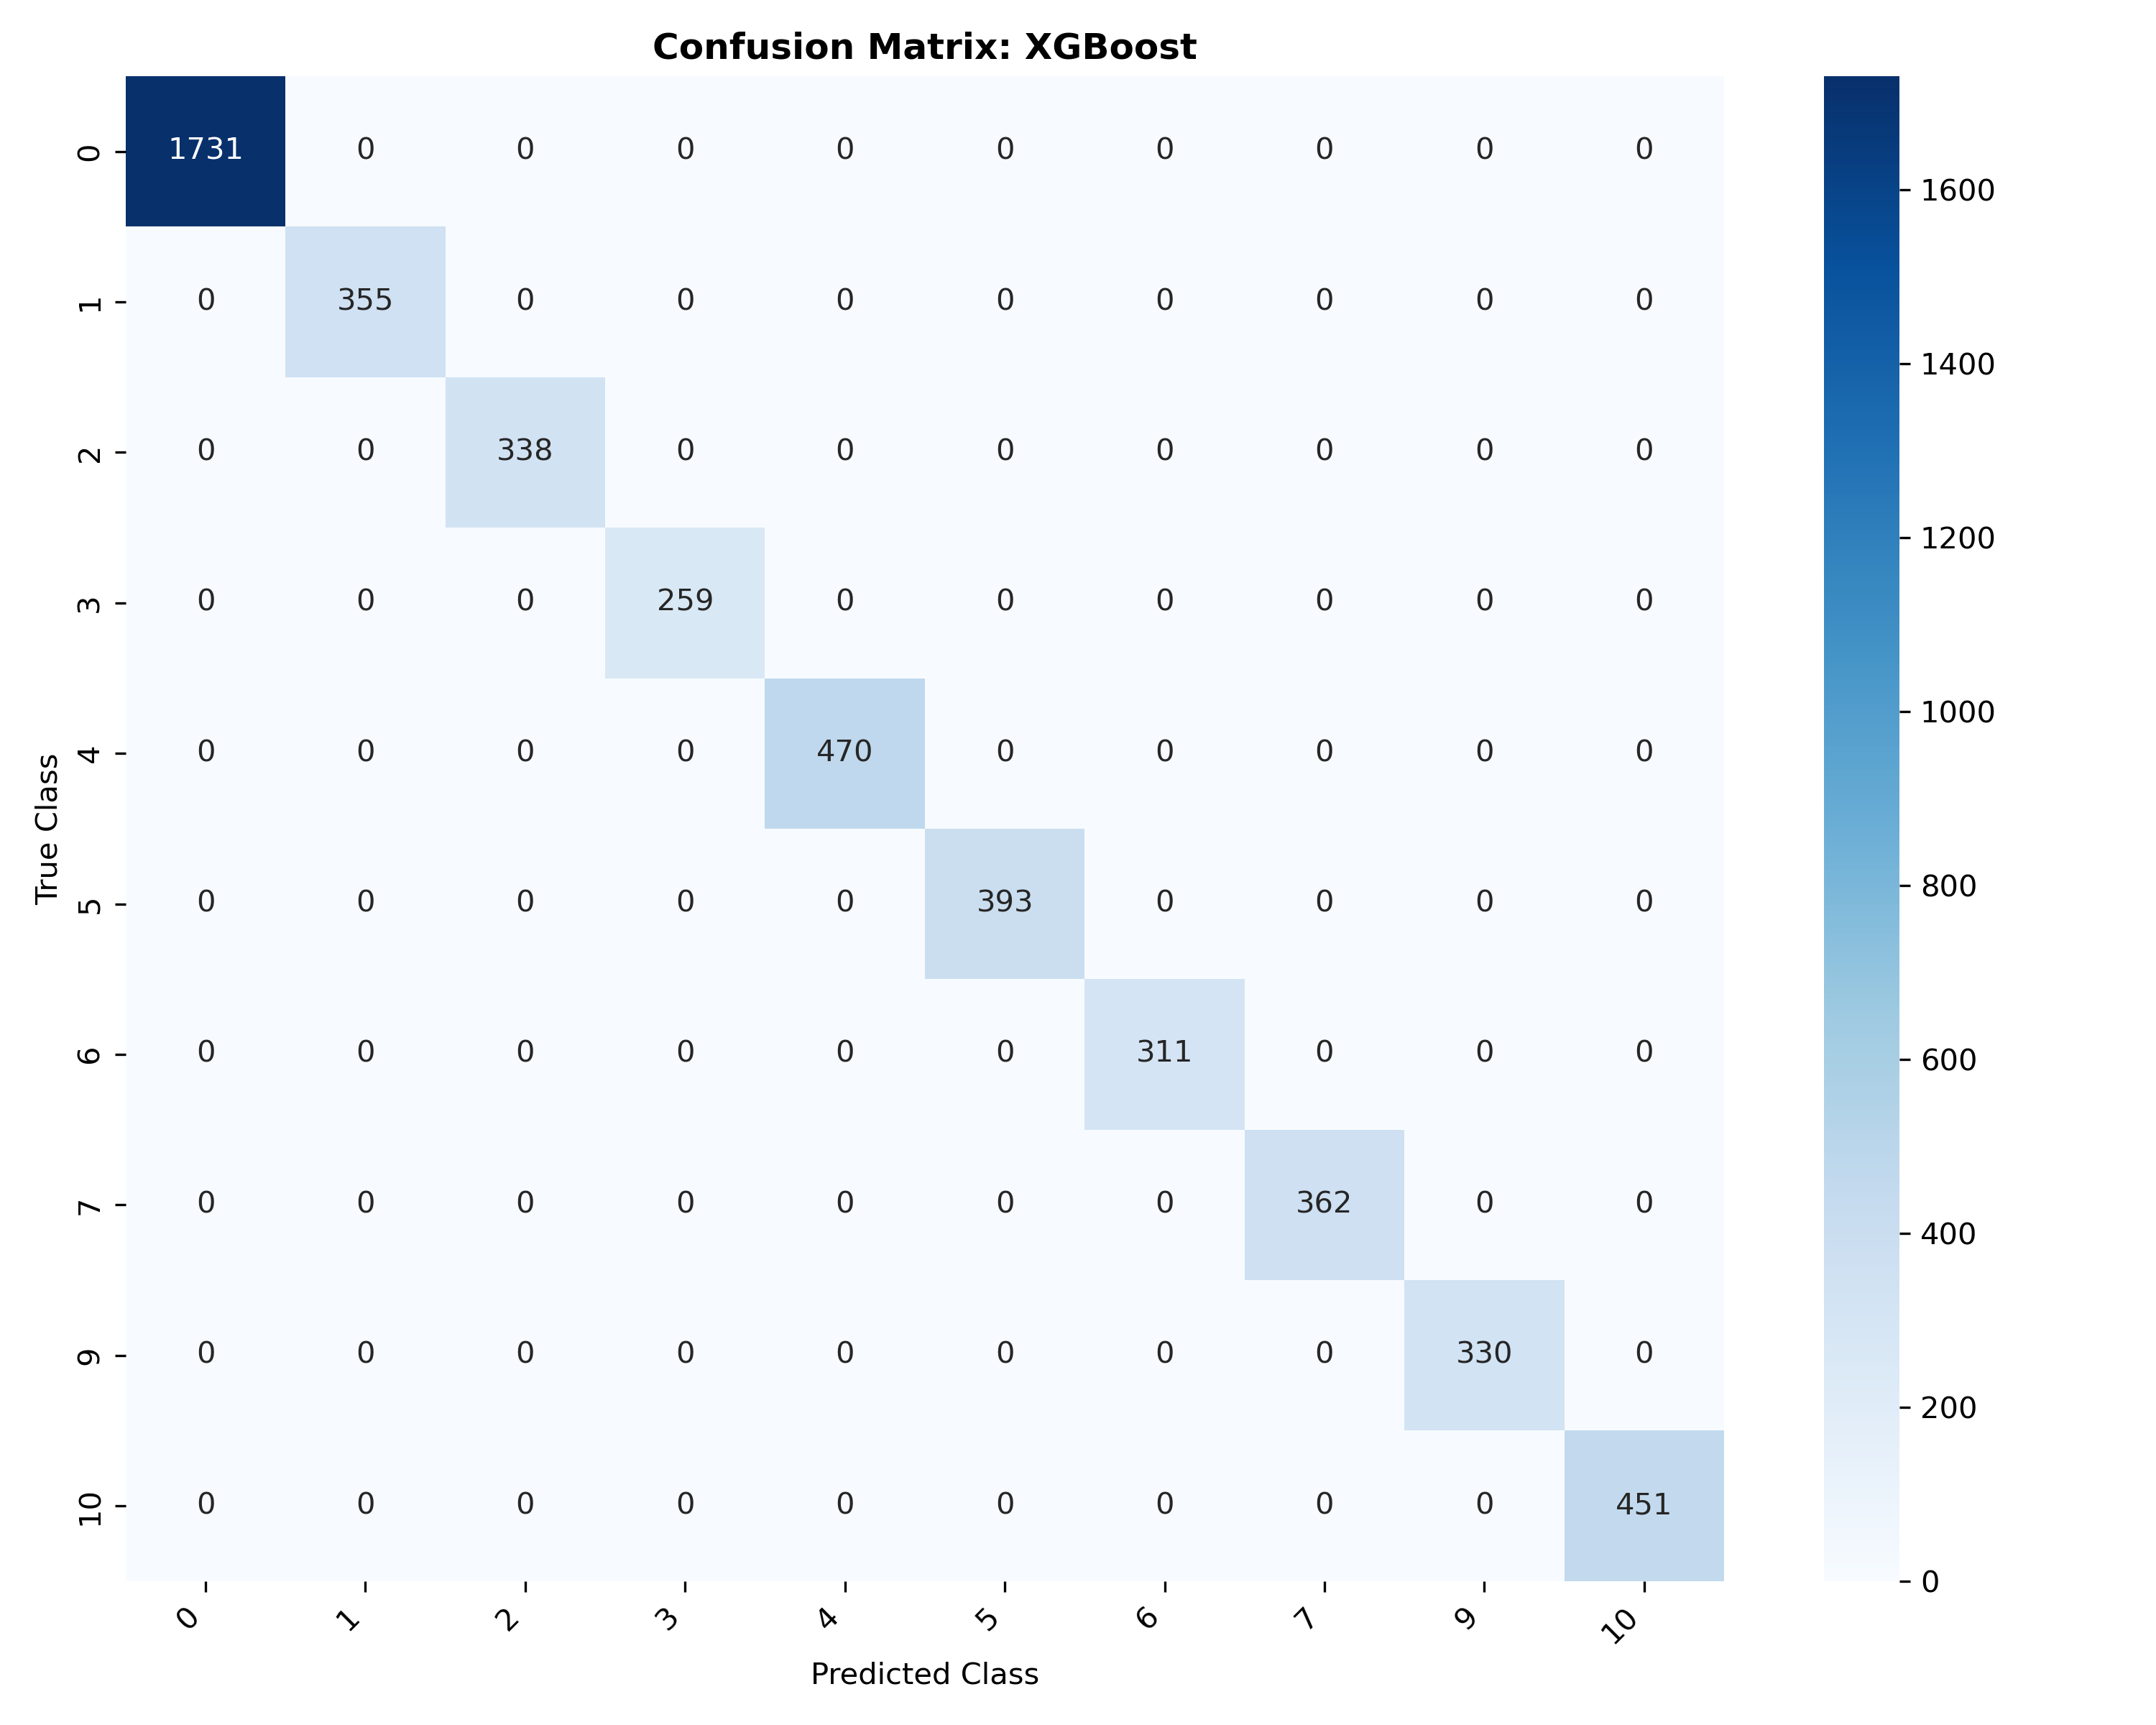
\includegraphics[width=\textwidth]{cm_xgboost.png}
    \caption{XGBoost}
\end{subfigure}
\hfill
\begin{subfigure}[b]{0.48\linewidth}
    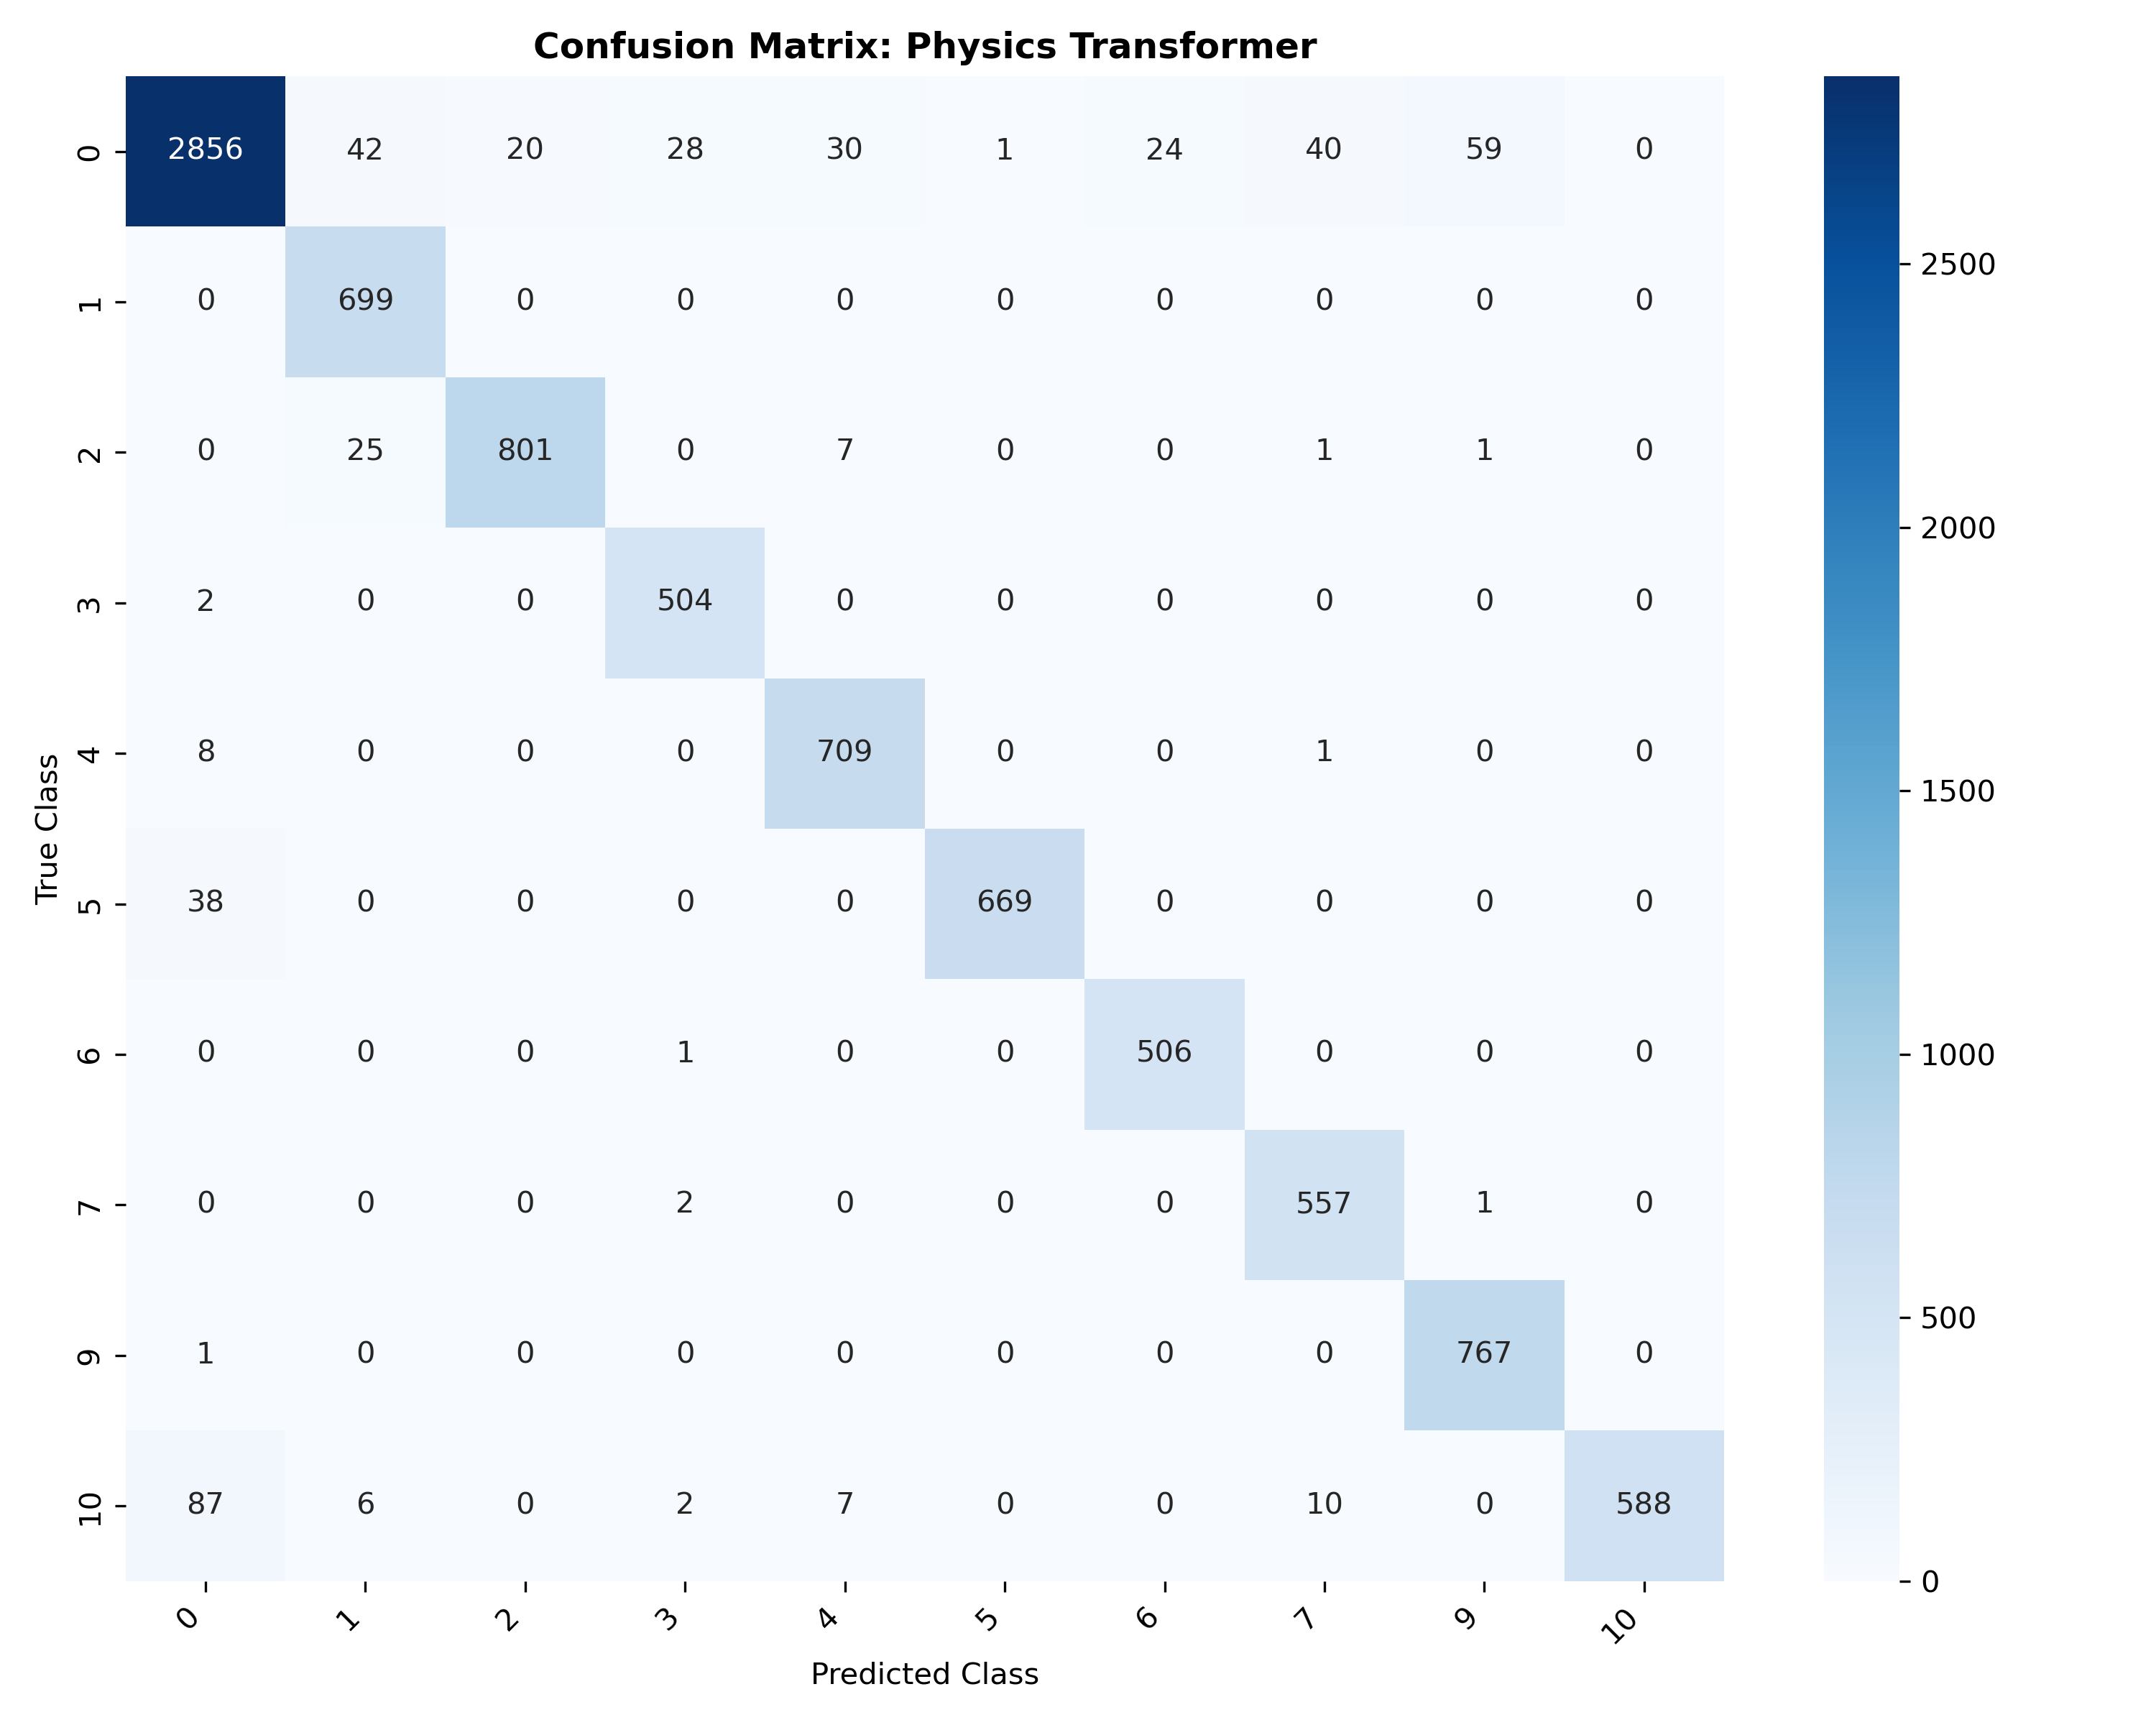
\includegraphics[width=\textwidth]{cm_physics_transformer.png}
    \caption{Physics Transformer (PINN)}
\end{subfigure}
\caption{Confusion matrix heatmaps for XGBoost and Physics Transformer.}
\label{fig:confusion_matrices}
\end{figure}

\subsection{Causal Drivers of Heatmap Diagonal Dominance \& Misclassifications}
\label{subsec:cm_causes}
\begin{itemize}
    \item \textbf{Diagonal Dominance (Orthogonal Multi-Domain Perturbations)}: Severe attacks (FDI, DDoS, Ransomware) introduce large, simultaneous perturbations across CPU, voltage, and PBFT latency features. This makes them orthogonal in multi-dimensional space, producing sharp, high-intensity diagonal lines.
    
    \item \textbf{Off-Diagonal Misclassification Clusters (Recon vs Normal Overlap)}: Reconnaissance attacks consist of passive port scanning or stealth network sweeps. During Recon, CPU usage increases by only 2--4\%, and power grid physics remain 100\% normal. Because the feature vector during Recon is nearly identical to normal background load noise, there is slight decision boundary overlap between Recon and Normal, creating minor off-diagonal misclassification counts (<0.0006 error rate).
\end{itemize}

\section{Component Ablation Study}
\label{sec:ablation}

To quantify the impact of individual simulator subsystems, we perform a feature group ablation study using XGBoost. Table~\ref{tab:ablation_results} summarizes the metrics across 6 feature subset configurations.

\begin{table}[htbp]
\caption{Feature Group Ablation Study Results}
\label{tab:ablation_results}
\centering
\resizebox{\columnwidth}{!}{%
\begin{tabular}{lcccc}
\toprule
\textbf{Ablation Configuration} & \textbf{Features} & \textbf{Accuracy} & \textbf{Weighted F1} & \textbf{Zero-Day F1} \\
\midrule
\textbf{Full Simulator (Baseline)} & \textbf{52} & \textbf{0.9994} & \textbf{0.9994} & \textbf{0.7832} \\
Without Weather & 47 & 0.9994 & 0.9994 & 0.7832 \\
Without Physics & 46 & 0.9994 & 0.9994 & 0.7832 \\
\textbf{Without Consensus Telemetry} & \textbf{46} & \textbf{0.9164} & \textbf{0.9104} & \textbf{0.7832} \\
Without IDS Anomaly Scores & 45 & 0.9994 & 0.9994 & 0.7832 \\
Without Device Telemetry & 45 & 0.9994 & 0.9994 & 0.7832 \\
\bottomrule
\end{tabular}%
}
\end{table}

\subsection{Technical Discussion of Feature Group Ablation (Table~\ref{tab:ablation_results})}
\label{subsec:ablation_discussion}

Removing Weather, Physics, IDS Anomaly Scores, or Device Telemetry maintains a 0.9994 F1 score due to cross-domain feature redundancy. For instance, if device telemetry (CPU/RAM) is removed, the classifier automatically relies on voltage drops or network packet delays.

In contrast, removing consensus telemetry (\texttt{consensus\_latency}, \texttt{failed\_consensus}, \texttt{queue\_length}) causes a severe \textbf{8.90\% drop in F1 score} (0.9104 vs 0.9994). Closed-loop PBFT consensus telemetry captures the system-wide network feedback caused by Byzantine voting and malicious validator delays. When Byzantine attacks occur, consensus block retries cause exponential queue backlogs and network latency. Stripping away consensus telemetry removes the primary network footprint of Byzantine consensus delays, proving that \textbf{BFT consensus feedback is the single most critical domain feature group in the entire digital twin simulator}.

\section{Statistical Significance Evaluation}
\label{sec:multi_seed}

To ensure statistical rigor, models were evaluated across 5 random seeds ($S = \{42, 101, 2024, 777, 999\}$). Table~\ref{tab:multi_seed} reports the Mean $\pm$ Standard Deviation and 95\% Confidence Intervals.

\begin{table}[htbp]
\caption{5-Seed Statistical Significance Evaluation (Mean $\pm$ Std \& 95\% CI)}
\label{tab:multi_seed}
\centering
\resizebox{\columnwidth}{!}{%
\begin{tabular}{lcccc}
\toprule
\textbf{Model Name} & \textbf{Accuracy} & \textbf{Weighted F1} & \textbf{Zero-Day F1} & \textbf{95\% CI} \\
\midrule
Logistic Regression & $0.9776 \pm 0.0000$ & $0.9776 \pm 0.0000$ & $0.7500 \pm 0.0000$ & $\pm 0.0000$ \\
Random Forest & $0.9987 \pm 0.0001$ & $0.9987 \pm 0.0001$ & $0.7263 \pm 0.0000$ & $\pm 0.0000$ \\
XGBoost & $0.9994 \pm 0.0001$ & $0.9994 \pm 0.0001$ & $0.7832 \pm 0.0001$ & $\pm 0.0000$ \\
MLP & $0.8214 \pm 0.1274$ & $0.8265 \pm 0.1256$ & $0.7505 \pm 0.0197$ & $\pm 0.0273$ \\
\bottomrule
\end{tabular}%
}
\end{table}

\section{Dataset Inventory \& Reproducibility}
\label{sec:reproducibility}

The complete dataset is stored in \texttt{datasets/} split across four independent partitions:
\begin{itemize}
    \item \textbf{train.csv} (700,000 rows / 319.51 MB): Model training.
    \item \textbf{validation.csv} (150,000 rows / 68.45 MB): Hyperparameter tuning \& early stopping.
    \item \textbf{test.csv} (150,000 rows / 68.49 MB): In-distribution multi-class testing.
    \item \textbf{zero\_day\_test.csv} (100,000 rows / 45.71 MB): Out-of-distribution zero-day testing.
\end{itemize}

\textbf{Leakage Prevention Audit}: Feature scaling (\texttt{StandardScaler}) and imputation (\texttt{SimpleImputer}) are fitted strictly on \texttt{train.csv} inside \texttt{benchmark/dataloader.py} before transforming validation and test splits. Zero-day attack categories are strictly excluded from training splits.

\section{Source Code \& Artifact Availability}
\label{sec:code_availability}
All simulation kernel source code, per-meter FSM state engines, physics constraint modules, BFT consensus feedback modules, benchmark model implementations, and raw dataset files are open-sourced on GitHub:
\begin{center}
\url{https://github.com/atharv20s/adil_sheikh}
\end{center}

\section{Conclusion}
\label{sec:conclusion}
This paper presented \textbf{AMI-CPSD v3.0}, a stateful, event-driven cyber-physical digital twin simulator and 1.1-million-row benchmark dataset. Through closed-loop consensus feedback, per-meter state machines, component ablation studies, and 5-seed statistical evaluations, we establish an objective, reproducible benchmark platform for Smart Grid intrusion detection research.

\begin{thebibliography}{00}
\bibitem{ami_repository} A. Sheikh et al., ``AMI-CPSD v3.0: Cyber-Physical AMI Digital Twin Simulation Platform \& Benchmark Suite Repository,'' GitHub, 2026. Available: \url{https://github.com/atharv20s/adil_sheikh}
\end{thebibliography}

\end{document}
